% Options for packages loaded elsewhere
\PassOptionsToPackage{unicode}{hyperref}
\PassOptionsToPackage{hyphens}{url}
\PassOptionsToPackage{dvipsnames,svgnames,x11names}{xcolor}
%
\documentclass[
  letterpaper,
  DIV=11,
  numbers=noendperiod]{scrartcl}

\usepackage{amsmath,amssymb}
\usepackage{iftex}
\ifPDFTeX
  \usepackage[T1]{fontenc}
  \usepackage[utf8]{inputenc}
  \usepackage{textcomp} % provide euro and other symbols
\else % if luatex or xetex
  \usepackage{unicode-math}
  \defaultfontfeatures{Scale=MatchLowercase}
  \defaultfontfeatures[\rmfamily]{Ligatures=TeX,Scale=1}
\fi
\usepackage{lmodern}
\ifPDFTeX\else  
    % xetex/luatex font selection
\fi
% Use upquote if available, for straight quotes in verbatim environments
\IfFileExists{upquote.sty}{\usepackage{upquote}}{}
\IfFileExists{microtype.sty}{% use microtype if available
  \usepackage[]{microtype}
  \UseMicrotypeSet[protrusion]{basicmath} % disable protrusion for tt fonts
}{}
\makeatletter
\@ifundefined{KOMAClassName}{% if non-KOMA class
  \IfFileExists{parskip.sty}{%
    \usepackage{parskip}
  }{% else
    \setlength{\parindent}{0pt}
    \setlength{\parskip}{6pt plus 2pt minus 1pt}}
}{% if KOMA class
  \KOMAoptions{parskip=half}}
\makeatother
\usepackage{xcolor}
\setlength{\emergencystretch}{3em} % prevent overfull lines
\setcounter{secnumdepth}{-\maxdimen} % remove section numbering
% Make \paragraph and \subparagraph free-standing
\makeatletter
\ifx\paragraph\undefined\else
  \let\oldparagraph\paragraph
  \renewcommand{\paragraph}{
    \@ifstar
      \xxxParagraphStar
      \xxxParagraphNoStar
  }
  \newcommand{\xxxParagraphStar}[1]{\oldparagraph*{#1}\mbox{}}
  \newcommand{\xxxParagraphNoStar}[1]{\oldparagraph{#1}\mbox{}}
\fi
\ifx\subparagraph\undefined\else
  \let\oldsubparagraph\subparagraph
  \renewcommand{\subparagraph}{
    \@ifstar
      \xxxSubParagraphStar
      \xxxSubParagraphNoStar
  }
  \newcommand{\xxxSubParagraphStar}[1]{\oldsubparagraph*{#1}\mbox{}}
  \newcommand{\xxxSubParagraphNoStar}[1]{\oldsubparagraph{#1}\mbox{}}
\fi
\makeatother

\usepackage{color}
\usepackage{fancyvrb}
\newcommand{\VerbBar}{|}
\newcommand{\VERB}{\Verb[commandchars=\\\{\}]}
\DefineVerbatimEnvironment{Highlighting}{Verbatim}{commandchars=\\\{\}}
% Add ',fontsize=\small' for more characters per line
\usepackage{framed}
\definecolor{shadecolor}{RGB}{241,243,245}
\newenvironment{Shaded}{\begin{snugshade}}{\end{snugshade}}
\newcommand{\AlertTok}[1]{\textcolor[rgb]{0.68,0.00,0.00}{#1}}
\newcommand{\AnnotationTok}[1]{\textcolor[rgb]{0.37,0.37,0.37}{#1}}
\newcommand{\AttributeTok}[1]{\textcolor[rgb]{0.40,0.45,0.13}{#1}}
\newcommand{\BaseNTok}[1]{\textcolor[rgb]{0.68,0.00,0.00}{#1}}
\newcommand{\BuiltInTok}[1]{\textcolor[rgb]{0.00,0.23,0.31}{#1}}
\newcommand{\CharTok}[1]{\textcolor[rgb]{0.13,0.47,0.30}{#1}}
\newcommand{\CommentTok}[1]{\textcolor[rgb]{0.37,0.37,0.37}{#1}}
\newcommand{\CommentVarTok}[1]{\textcolor[rgb]{0.37,0.37,0.37}{\textit{#1}}}
\newcommand{\ConstantTok}[1]{\textcolor[rgb]{0.56,0.35,0.01}{#1}}
\newcommand{\ControlFlowTok}[1]{\textcolor[rgb]{0.00,0.23,0.31}{\textbf{#1}}}
\newcommand{\DataTypeTok}[1]{\textcolor[rgb]{0.68,0.00,0.00}{#1}}
\newcommand{\DecValTok}[1]{\textcolor[rgb]{0.68,0.00,0.00}{#1}}
\newcommand{\DocumentationTok}[1]{\textcolor[rgb]{0.37,0.37,0.37}{\textit{#1}}}
\newcommand{\ErrorTok}[1]{\textcolor[rgb]{0.68,0.00,0.00}{#1}}
\newcommand{\ExtensionTok}[1]{\textcolor[rgb]{0.00,0.23,0.31}{#1}}
\newcommand{\FloatTok}[1]{\textcolor[rgb]{0.68,0.00,0.00}{#1}}
\newcommand{\FunctionTok}[1]{\textcolor[rgb]{0.28,0.35,0.67}{#1}}
\newcommand{\ImportTok}[1]{\textcolor[rgb]{0.00,0.46,0.62}{#1}}
\newcommand{\InformationTok}[1]{\textcolor[rgb]{0.37,0.37,0.37}{#1}}
\newcommand{\KeywordTok}[1]{\textcolor[rgb]{0.00,0.23,0.31}{\textbf{#1}}}
\newcommand{\NormalTok}[1]{\textcolor[rgb]{0.00,0.23,0.31}{#1}}
\newcommand{\OperatorTok}[1]{\textcolor[rgb]{0.37,0.37,0.37}{#1}}
\newcommand{\OtherTok}[1]{\textcolor[rgb]{0.00,0.23,0.31}{#1}}
\newcommand{\PreprocessorTok}[1]{\textcolor[rgb]{0.68,0.00,0.00}{#1}}
\newcommand{\RegionMarkerTok}[1]{\textcolor[rgb]{0.00,0.23,0.31}{#1}}
\newcommand{\SpecialCharTok}[1]{\textcolor[rgb]{0.37,0.37,0.37}{#1}}
\newcommand{\SpecialStringTok}[1]{\textcolor[rgb]{0.13,0.47,0.30}{#1}}
\newcommand{\StringTok}[1]{\textcolor[rgb]{0.13,0.47,0.30}{#1}}
\newcommand{\VariableTok}[1]{\textcolor[rgb]{0.07,0.07,0.07}{#1}}
\newcommand{\VerbatimStringTok}[1]{\textcolor[rgb]{0.13,0.47,0.30}{#1}}
\newcommand{\WarningTok}[1]{\textcolor[rgb]{0.37,0.37,0.37}{\textit{#1}}}

\providecommand{\tightlist}{%
  \setlength{\itemsep}{0pt}\setlength{\parskip}{0pt}}\usepackage{longtable,booktabs,array}
\usepackage{calc} % for calculating minipage widths
% Correct order of tables after \paragraph or \subparagraph
\usepackage{etoolbox}
\makeatletter
\patchcmd\longtable{\par}{\if@noskipsec\mbox{}\fi\par}{}{}
\makeatother
% Allow footnotes in longtable head/foot
\IfFileExists{footnotehyper.sty}{\usepackage{footnotehyper}}{\usepackage{footnote}}
\makesavenoteenv{longtable}
\usepackage{graphicx}
\makeatletter
\def\maxwidth{\ifdim\Gin@nat@width>\linewidth\linewidth\else\Gin@nat@width\fi}
\def\maxheight{\ifdim\Gin@nat@height>\textheight\textheight\else\Gin@nat@height\fi}
\makeatother
% Scale images if necessary, so that they will not overflow the page
% margins by default, and it is still possible to overwrite the defaults
% using explicit options in \includegraphics[width, height, ...]{}
\setkeys{Gin}{width=\maxwidth,height=\maxheight,keepaspectratio}
% Set default figure placement to htbp
\makeatletter
\def\fps@figure{htbp}
\makeatother

\usepackage{fvextra}
\DefineVerbatimEnvironment{Highlighting}{Verbatim}{breaklines,commandchars=\\\{\}}
\KOMAoption{captions}{tableheading}
\makeatletter
\@ifpackageloaded{caption}{}{\usepackage{caption}}
\AtBeginDocument{%
\ifdefined\contentsname
  \renewcommand*\contentsname{Table of contents}
\else
  \newcommand\contentsname{Table of contents}
\fi
\ifdefined\listfigurename
  \renewcommand*\listfigurename{List of Figures}
\else
  \newcommand\listfigurename{List of Figures}
\fi
\ifdefined\listtablename
  \renewcommand*\listtablename{List of Tables}
\else
  \newcommand\listtablename{List of Tables}
\fi
\ifdefined\figurename
  \renewcommand*\figurename{Figure}
\else
  \newcommand\figurename{Figure}
\fi
\ifdefined\tablename
  \renewcommand*\tablename{Table}
\else
  \newcommand\tablename{Table}
\fi
}
\@ifpackageloaded{float}{}{\usepackage{float}}
\floatstyle{ruled}
\@ifundefined{c@chapter}{\newfloat{codelisting}{h}{lop}}{\newfloat{codelisting}{h}{lop}[chapter]}
\floatname{codelisting}{Listing}
\newcommand*\listoflistings{\listof{codelisting}{List of Listings}}
\makeatother
\makeatletter
\makeatother
\makeatletter
\@ifpackageloaded{caption}{}{\usepackage{caption}}
\@ifpackageloaded{subcaption}{}{\usepackage{subcaption}}
\makeatother

\ifLuaTeX
  \usepackage{selnolig}  % disable illegal ligatures
\fi
\usepackage{bookmark}

\IfFileExists{xurl.sty}{\usepackage{xurl}}{} % add URL line breaks if available
\urlstyle{same} % disable monospaced font for URLs
\hypersetup{
  pdftitle={PS4},
  colorlinks=true,
  linkcolor={blue},
  filecolor={Maroon},
  citecolor={Blue},
  urlcolor={Blue},
  pdfcreator={LaTeX via pandoc}}


\title{PS4}
\author{}
\date{}

\begin{document}
\maketitle

\RecustomVerbatimEnvironment{verbatim}{Verbatim}{
  showspaces = false,
  showtabs = false,
  breaksymbolleft={},
  breaklines
}


\textbf{PS4:} Due Sat Nov 2 at 5:00PM Central. Worth 100 points. We use
(\texttt{*}) to indicate a problem that we think might be time
consuming.

\subsection{Style Points (10 pts)}\label{style-points-10-pts}

Please refer to the minilesson on code style
\textbf{\href{https://uchicago.zoom.us/rec/share/pG_wQ-pHTQrJTmqNn4rcrw5V194M2H2s-2jdy8oVhWHkd_yZt9o162IWurpA-fxU.BIQlSgZLRYctvzp-}{here}}.

\subsection{Submission Steps (10 pts)}\label{submission-steps-10-pts}

\begin{enumerate}
\def\labelenumi{\arabic{enumi}.}
\tightlist
\item
  This problem set is a paired problem set.
\item
  Play paper, scissors, rock to determine who goes first. Call that
  person \emph{Partner 1}.

  \begin{itemize}
  \tightlist
  \item
    Partner 1 (name and cnet ID): Duoshu Xu, duoshu
  \item
    Partner 2 (name and cnet ID): Jae Hu, jaehu
  \end{itemize}
\item
  Partner 1 will accept the \texttt{ps4} and then share the link it
  creates with their partner. You can only share it with one partner so
  you will not be able to change it after your partner has accepted.
\item
  ``This submission is our work alone and complies with the 30538
  integrity policy.'' Add your initials to indicate your agreement: JH
  DX
\item
  ``I have uploaded the names of anyone else other than my partner and I
  worked with on the problem set
  \textbf{\href{https://docs.google.com/forms/d/185usrCREQaUbvAXpWhChkjghdGgmAZXA3lPWpXLLsts/edit}{here}}''
  (1 point)
\item
  Late coins used this pset: 0 Late coins left after submission: 3
\item
  Knit your \texttt{ps4.qmd} to an PDF file to make \texttt{ps4.pdf},

  \begin{itemize}
  \tightlist
  \item
    The PDF should not be more than 25 pages. Use \texttt{head()} and
    re-size figures when appropriate.
  \end{itemize}
\item
  (Partner 1): push \texttt{ps4.qmd} and \texttt{ps4.pdf} to your github
  repo.
\item
  (Partner 1): submit \texttt{ps4.pdf} via Gradescope. Add your partner
  on Gradescope.
\item
  (Partner 1): tag your submission in Gradescope
\end{enumerate}

\textbf{Important:} Repositories are for tracking code. \textbf{Do not
commit the data or shapefiles to your repo.} The best way to do this is
with \texttt{.gitignore}, which we have covered in class. If you do
accidentally commit the data, Github has a
\href{https://docs.github.com/en/repositories/working-with-files/managing-large-files/about-large-files-on-github\#removing-files-from-a-repositorys-history}{guide}.
The best course of action depends on whether you have pushed yet. This
also means that both partners will have to download the initial raw data
and any data cleaning code will need to be re-run on both partners'
computers.

\subsection{Download and explore the Provider of Services (POS) file (10
pts)}\label{download-and-explore-the-provider-of-services-pos-file-10-pts}

\begin{enumerate}
\def\labelenumi{\arabic{enumi}.}
\tightlist
\item
\end{enumerate}

\begin{Shaded}
\begin{Highlighting}[]
\ImportTok{import}\NormalTok{ pandas }\ImportTok{as}\NormalTok{ pd}
\ImportTok{import}\NormalTok{ altair }\ImportTok{as}\NormalTok{ alt}
\ImportTok{import}\NormalTok{ geopandas }\ImportTok{as}\NormalTok{ gpd}
\ImportTok{import}\NormalTok{ matplotlib.pyplot }\ImportTok{as}\NormalTok{ plt}
\ImportTok{import}\NormalTok{ time}
\ImportTok{from}\NormalTok{ shapely.geometry }\ImportTok{import}\NormalTok{ Point}

\NormalTok{pos2016\_df }\OperatorTok{=}\NormalTok{ pd.read\_csv(}
    \StringTok{\textquotesingle{}/Users/kevinxu/Documents/GitHub/problem{-}set{-}4{-}xu{-}hu/pos2016.csv\textquotesingle{}}\NormalTok{,}
\NormalTok{    low\_memory}\OperatorTok{=}\VariableTok{False}
\NormalTok{)}
\NormalTok{pos2016\_df.head()}
\end{Highlighting}
\end{Shaded}

\begin{longtable}[]{@{}lllllllllllll@{}}
\toprule\noalign{}
& PRVDR\_CTGRY\_SBTYP\_CD & PRVDR\_CTGRY\_CD & SSA\_CNTY\_CD &
CRTFCTN\_DT & FAC\_NAME & PRVDR\_NUM & RGN\_CD & STATE\_CD & ST\_ADR &
PGM\_TRMNTN\_CD & GNRL\_CNTL\_TYPE\_CD & ZIP\_CD \\
\midrule\noalign{}
\endhead
\bottomrule\noalign{}
\endlastfoot
0 & 1.0 & 1 & 340 & 20000814 & SOUTHEAST ALABAMA MEDICAL CENTER & 010001
& 4 & AL & 1108 ROSS CLARK CIRCLE & 0 & 08 & 36301.0 \\
1 & 1.0 & 1 & 350 & 20010316 & NORTH JACKSON HOSPITAL & 010004 & 4 & AL
& 47005 U S HIGHWAY 72 & 1 & 08 & 35740.0 \\
2 & 1.0 & 1 & 470 & 20021003 & MARSHALL MEDICAL CENTER SOUTH & 010005 &
4 & AL & 2505 U S HIGHWAY 431 NORTH & 0 & 08 & 35957.0 \\
3 & 1.0 & 1 & 380 & 20100715 & ELIZA COFFEE MEMORIAL HOSPITAL & 010006 &
4 & AL & 205 MARENGO STREET & 0 & 08 & 35631.0 \\
4 & 1.0 & 1 & 190 & 20150716 & MIZELL MEMORIAL HOSPITAL & 010007 & 4 &
AL & 702 N MAIN ST & 0 & 02 & 36467.0 \\
\end{longtable}

The variables we pulled are: PRVDR\_CTGRY\_SBTYP\_CD - Provider Category
Subtype Code PRVDR\_CTGRY\_CD - Provider Category Code SSA\_CNTY\_CD -
SSA County Code CRTFCTN\_DT - Certification Date FAC\_NAME - Facility
Name PRVDR\_NUM - CMS Certification Number RGN\_CD - Region Code
STATE\_CD - State Abbreviation ST\_ADR - Street Address PGM\_TRMNTN\_CD
- Termination Code GNRL\_CNTL\_TYPE\_CD - General Control Type Code
ZIP\_CD - ZIP Code

\begin{enumerate}
\def\labelenumi{\arabic{enumi}.}
\setcounter{enumi}{1}
\tightlist
\item
\end{enumerate}

\begin{Shaded}
\begin{Highlighting}[]
\NormalTok{short\_term\_2016 }\OperatorTok{=}\NormalTok{ pos2016\_df[(pos2016\_df[}\StringTok{\textquotesingle{}PRVDR\_CTGRY\_CD\textquotesingle{}}\NormalTok{] }\OperatorTok{==} \DecValTok{1}\NormalTok{) }\OperatorTok{\&}\NormalTok{ (}
\NormalTok{    pos2016\_df[}\StringTok{\textquotesingle{}PRVDR\_CTGRY\_SBTYP\_CD\textquotesingle{}}\NormalTok{] }\OperatorTok{==} \DecValTok{1}\NormalTok{)]}
\NormalTok{num\_short\_term\_hospitals }\OperatorTok{=}\NormalTok{ short\_term\_2016.shape[}\DecValTok{0}\NormalTok{]}
\NormalTok{num\_short\_term\_hospitals}
\end{Highlighting}
\end{Shaded}

\begin{verbatim}
7245
\end{verbatim}

The number of hospitals reported in this data is 7245. This number seems
higher than estimates from other sources. For example, according to the
American Hospital Association's 2017 report:
https://www.aha.org/system/files/2018-01/Fast\%20Facts\%202018\%20pie\%20charts.pdf
there are 5,534 hospitals in the US in 2016. Some possible reasons for
the discrapancy: the CMS data might include specialized hospitals, such
as psychiatric hospitals, that might not be included by the AHA. It is
also possible that some hospitals have multiple CMS certification
numbers due to mergers or acquisitions.

\begin{enumerate}
\def\labelenumi{\arabic{enumi}.}
\setcounter{enumi}{2}
\tightlist
\item
\end{enumerate}

\begin{Shaded}
\begin{Highlighting}[]
\NormalTok{pos2017\_df }\OperatorTok{=}\NormalTok{ pd.read\_csv(}
    \StringTok{\textquotesingle{}/Users/kevinxu/Documents/GitHub/problem{-}set{-}4{-}xu{-}hu/pos2017.csv\textquotesingle{}}\NormalTok{, encoding}\OperatorTok{=}\StringTok{\textquotesingle{}latin1\textquotesingle{}}\NormalTok{, low\_memory}\OperatorTok{=}\VariableTok{False}\NormalTok{)}
\NormalTok{pos2018\_df }\OperatorTok{=}\NormalTok{ pd.read\_csv(}
    \StringTok{\textquotesingle{}/Users/kevinxu/Documents/GitHub/problem{-}set{-}4{-}xu{-}hu/pos2018.csv\textquotesingle{}}\NormalTok{, encoding}\OperatorTok{=}\StringTok{\textquotesingle{}latin1\textquotesingle{}}\NormalTok{, low\_memory}\OperatorTok{=}\VariableTok{False}\NormalTok{)}
\NormalTok{pos2019\_df }\OperatorTok{=}\NormalTok{ pd.read\_csv(}
    \StringTok{\textquotesingle{}/Users/kevinxu/Documents/GitHub/problem{-}set{-}4{-}xu{-}hu/pos2019.csv\textquotesingle{}}\NormalTok{, encoding}\OperatorTok{=}\StringTok{\textquotesingle{}latin1\textquotesingle{}}\NormalTok{, low\_memory}\OperatorTok{=}\VariableTok{False}\NormalTok{)}

\NormalTok{short\_term\_2017 }\OperatorTok{=}\NormalTok{ pos2017\_df[(pos2017\_df[}\StringTok{\textquotesingle{}PRVDR\_CTGRY\_CD\textquotesingle{}}\NormalTok{] }\OperatorTok{==} \DecValTok{1}\NormalTok{) }\OperatorTok{\&}\NormalTok{ (}
\NormalTok{    pos2017\_df[}\StringTok{\textquotesingle{}PRVDR\_CTGRY\_SBTYP\_CD\textquotesingle{}}\NormalTok{] }\OperatorTok{==} \DecValTok{1}\NormalTok{)]}
\NormalTok{pos2018\_df.rename(}
\NormalTok{    columns}\OperatorTok{=}\NormalTok{\{}\StringTok{\textquotesingle{}PRVDR\_CTGRY\_SBTYP\_CD\textquotesingle{}}\NormalTok{: }\StringTok{\textquotesingle{}PRVDR\_CTGRY\_SBTYP\_CD\textquotesingle{}}\NormalTok{\}, inplace}\OperatorTok{=}\VariableTok{True}\NormalTok{)}
\NormalTok{short\_term\_2018 }\OperatorTok{=}\NormalTok{ pos2018\_df[(pos2018\_df[}\StringTok{\textquotesingle{}PRVDR\_CTGRY\_CD\textquotesingle{}}\NormalTok{] }\OperatorTok{==} \DecValTok{1}\NormalTok{) }\OperatorTok{\&}\NormalTok{ (}
\NormalTok{    pos2018\_df[}\StringTok{\textquotesingle{}PRVDR\_CTGRY\_SBTYP\_CD\textquotesingle{}}\NormalTok{] }\OperatorTok{==} \DecValTok{1}\NormalTok{)]}
\NormalTok{short\_term\_2019 }\OperatorTok{=}\NormalTok{ pos2019\_df[(pos2019\_df[}\StringTok{\textquotesingle{}PRVDR\_CTGRY\_CD\textquotesingle{}}\NormalTok{] }\OperatorTok{==} \DecValTok{1}\NormalTok{) }\OperatorTok{\&}\NormalTok{ (}
\NormalTok{    pos2019\_df[}\StringTok{\textquotesingle{}PRVDR\_CTGRY\_SBTYP\_CD\textquotesingle{}}\NormalTok{] }\OperatorTok{==} \DecValTok{1}\NormalTok{)]}

\NormalTok{all\_short\_term\_hospitals }\OperatorTok{=}\NormalTok{ pd.concat(}
\NormalTok{    [short\_term\_2016, short\_term\_2017, short\_term\_2018, short\_term\_2019], axis}\OperatorTok{=}\DecValTok{0}\NormalTok{)}

\NormalTok{total\_short\_term\_hospitals }\OperatorTok{=}\NormalTok{ all\_short\_term\_hospitals.shape[}\DecValTok{0}\NormalTok{]}

\BuiltInTok{print}\NormalTok{(}\StringTok{"Total number of short{-}term hospitals from 2016 to 2019:"}\NormalTok{,}
\NormalTok{      total\_short\_term\_hospitals)}
\end{Highlighting}
\end{Shaded}

\begin{verbatim}
Total number of short-term hospitals from 2016 to 2019: 29085
\end{verbatim}

\begin{Shaded}
\begin{Highlighting}[]
\NormalTok{short\_term\_2016 }\OperatorTok{=}\NormalTok{ short\_term\_2016.copy()}
\NormalTok{short\_term\_2016[}\StringTok{\textquotesingle{}Year\textquotesingle{}}\NormalTok{] }\OperatorTok{=} \DecValTok{2016}
\NormalTok{short\_term\_2017 }\OperatorTok{=}\NormalTok{ short\_term\_2017.copy()}
\NormalTok{short\_term\_2017[}\StringTok{\textquotesingle{}Year\textquotesingle{}}\NormalTok{] }\OperatorTok{=} \DecValTok{2017}
\NormalTok{short\_term\_2018 }\OperatorTok{=}\NormalTok{ short\_term\_2018.copy()}
\NormalTok{short\_term\_2018[}\StringTok{\textquotesingle{}Year\textquotesingle{}}\NormalTok{] }\OperatorTok{=} \DecValTok{2018}
\NormalTok{short\_term\_2019 }\OperatorTok{=}\NormalTok{ short\_term\_2019.copy()}
\NormalTok{short\_term\_2019[}\StringTok{\textquotesingle{}Year\textquotesingle{}}\NormalTok{] }\OperatorTok{=} \DecValTok{2019}

\NormalTok{all\_short\_term\_hospitals }\OperatorTok{=}\NormalTok{ pd.concat(}
\NormalTok{    [short\_term\_2016, short\_term\_2017, short\_term\_2018, short\_term\_2019], axis}\OperatorTok{=}\DecValTok{0}\NormalTok{)}
\NormalTok{observations\_by\_year }\OperatorTok{=}\NormalTok{ all\_short\_term\_hospitals[}\StringTok{\textquotesingle{}Year\textquotesingle{}}\NormalTok{].value\_counts(}
\NormalTok{).sort\_index()}

\NormalTok{observations\_data }\OperatorTok{=}\NormalTok{ pd.DataFrame(\{}
    \StringTok{\textquotesingle{}Year\textquotesingle{}}\NormalTok{: observations\_by\_year.index,}
    \StringTok{\textquotesingle{}Number of Observations\textquotesingle{}}\NormalTok{: observations\_by\_year.values}
\NormalTok{\})}

\NormalTok{chart }\OperatorTok{=}\NormalTok{ alt.Chart(observations\_data).mark\_bar().encode(}
\NormalTok{    x}\OperatorTok{=}\NormalTok{alt.X(}\StringTok{\textquotesingle{}Year:O\textquotesingle{}}\NormalTok{, title}\OperatorTok{=}\StringTok{\textquotesingle{}Year\textquotesingle{}}\NormalTok{),}
\NormalTok{    y}\OperatorTok{=}\NormalTok{alt.Y(}\StringTok{\textquotesingle{}Number of Observations:Q\textquotesingle{}}\NormalTok{, title}\OperatorTok{=}\StringTok{\textquotesingle{}Number of Observations\textquotesingle{}}\NormalTok{),}
\NormalTok{    tooltip}\OperatorTok{=}\NormalTok{[}\StringTok{\textquotesingle{}Year\textquotesingle{}}\NormalTok{, }\StringTok{\textquotesingle{}Number of Observations\textquotesingle{}}\NormalTok{]}
\NormalTok{).properties(}
\NormalTok{    title}\OperatorTok{=}\StringTok{\textquotesingle{}Number of Short{-}term Hospital by Year (2016{-}2019)\textquotesingle{}}\NormalTok{,}
\NormalTok{    width}\OperatorTok{=}\DecValTok{500}\NormalTok{,}
\NormalTok{)}

\NormalTok{chart}
\end{Highlighting}
\end{Shaded}

\begin{verbatim}
alt.Chart(...)
\end{verbatim}

\begin{enumerate}
\def\labelenumi{\arabic{enumi}.}
\setcounter{enumi}{3}
\tightlist
\item
\end{enumerate}

\begin{Shaded}
\begin{Highlighting}[]
\NormalTok{unique\_hospitals\_by\_year }\OperatorTok{=}\NormalTok{ all\_short\_term\_hospitals.groupby(}\StringTok{\textquotesingle{}Year\textquotesingle{}}\NormalTok{)[}
    \StringTok{\textquotesingle{}PRVDR\_NUM\textquotesingle{}}\NormalTok{].nunique()}
\NormalTok{unique\_hospitals\_data }\OperatorTok{=}\NormalTok{ pd.DataFrame(\{}
    \StringTok{\textquotesingle{}Year\textquotesingle{}}\NormalTok{: unique\_hospitals\_by\_year.index,}
    \StringTok{\textquotesingle{}Number of Unique Hospitals\textquotesingle{}}\NormalTok{: unique\_hospitals\_by\_year.values}
\NormalTok{\})}

\NormalTok{unique\_hospitals\_chart }\OperatorTok{=}\NormalTok{ alt.Chart(unique\_hospitals\_data).mark\_bar(color}\OperatorTok{=}\StringTok{\textquotesingle{}blue\textquotesingle{}}\NormalTok{).encode(}
\NormalTok{    x}\OperatorTok{=}\NormalTok{alt.X(}\StringTok{\textquotesingle{}Year:O\textquotesingle{}}\NormalTok{, title}\OperatorTok{=}\StringTok{\textquotesingle{}Year\textquotesingle{}}\NormalTok{),}
\NormalTok{    y}\OperatorTok{=}\NormalTok{alt.Y(}\StringTok{\textquotesingle{}Number of Unique Hospitals:Q\textquotesingle{}}\NormalTok{,}
\NormalTok{            title}\OperatorTok{=}\StringTok{\textquotesingle{}Number of Unique Hospitals\textquotesingle{}}\NormalTok{),}
\NormalTok{    tooltip}\OperatorTok{=}\NormalTok{[}\StringTok{\textquotesingle{}Year\textquotesingle{}}\NormalTok{, }\StringTok{\textquotesingle{}Number of Unique Hospitals\textquotesingle{}}\NormalTok{]}
\NormalTok{).properties(}
\NormalTok{    title}\OperatorTok{=}\StringTok{\textquotesingle{}Number of Unique Short{-}term Hospitals by Year (2016{-}2019)\textquotesingle{}}\NormalTok{,}
\NormalTok{    width}\OperatorTok{=}\DecValTok{500}\NormalTok{,}
\NormalTok{)}

\NormalTok{unique\_hospitals\_chart}
\end{Highlighting}
\end{Shaded}

\begin{verbatim}
alt.Chart(...)
\end{verbatim}

The graphs from question 3 and question 4 are identical. This means that
the number of unique short-term hospitals is the same as the total
number of short-term hospitals. This suggests that each observation in
this dataset represents one unique facility instead of multiple entries
per hospital.

\subsection{Identify hospital closures in POS file (15 pts)
(*)}\label{identify-hospital-closures-in-pos-file-15-pts}

\begin{enumerate}
\def\labelenumi{\arabic{enumi}.}
\tightlist
\item
\end{enumerate}

\begin{Shaded}
\begin{Highlighting}[]
\NormalTok{active\_2016 }\OperatorTok{=}\NormalTok{ short\_term\_2016[short\_term\_2016[}\StringTok{\textquotesingle{}PGM\_TRMNTN\_CD\textquotesingle{}}\NormalTok{] }\OperatorTok{==} \DecValTok{0}\NormalTok{]}

\NormalTok{suspected\_closures }\OperatorTok{=}\NormalTok{ []}

\ControlFlowTok{for}\NormalTok{ index, hospital }\KeywordTok{in}\NormalTok{ active\_2016.iterrows():}
\NormalTok{    cms\_cert\_num }\OperatorTok{=}\NormalTok{ hospital[}\StringTok{\textquotesingle{}PRVDR\_NUM\textquotesingle{}}\NormalTok{]}
\NormalTok{    facility\_name }\OperatorTok{=}\NormalTok{ hospital[}\StringTok{\textquotesingle{}FAC\_NAME\textquotesingle{}}\NormalTok{]}
\NormalTok{    zip\_code }\OperatorTok{=}\NormalTok{ hospital[}\StringTok{\textquotesingle{}ZIP\_CD\textquotesingle{}}\NormalTok{]}

\NormalTok{    closed\_year }\OperatorTok{=} \VariableTok{None}

    \ControlFlowTok{for}\NormalTok{ year, dataset }\KeywordTok{in} \BuiltInTok{zip}\NormalTok{([}\DecValTok{2017}\NormalTok{, }\DecValTok{2018}\NormalTok{, }\DecValTok{2019}\NormalTok{], [short\_term\_2017, short\_term\_2018, short\_term\_2019]):}
\NormalTok{        hospital\_in\_year }\OperatorTok{=}\NormalTok{ dataset[dataset[}\StringTok{\textquotesingle{}PRVDR\_NUM\textquotesingle{}}\NormalTok{] }\OperatorTok{==}\NormalTok{ cms\_cert\_num]}
        \ControlFlowTok{if}\NormalTok{ hospital\_in\_year.empty }\KeywordTok{or}\NormalTok{ hospital\_in\_year.iloc[}\DecValTok{0}\NormalTok{][}\StringTok{\textquotesingle{}PGM\_TRMNTN\_CD\textquotesingle{}}\NormalTok{] }\OperatorTok{!=} \DecValTok{0}\NormalTok{:}
\NormalTok{            closed\_year }\OperatorTok{=}\NormalTok{ year}
            \ControlFlowTok{break}

    \ControlFlowTok{if}\NormalTok{ closed\_year:}
\NormalTok{        suspected\_closures.append(\{}
            \StringTok{\textquotesingle{}Facility Name\textquotesingle{}}\NormalTok{: facility\_name,}
            \StringTok{\textquotesingle{}ZIP Code\textquotesingle{}}\NormalTok{: zip\_code,}
            \StringTok{\textquotesingle{}Year of Suspected Closure\textquotesingle{}}\NormalTok{: closed\_year}
\NormalTok{        \})}

\NormalTok{suspected\_closures\_df }\OperatorTok{=}\NormalTok{ pd.DataFrame(suspected\_closures)}
\NormalTok{num\_suspected\_closures }\OperatorTok{=}\NormalTok{ suspected\_closures\_df.shape[}\DecValTok{0}\NormalTok{]}
\NormalTok{num\_suspected\_closures}
\end{Highlighting}
\end{Shaded}

\begin{verbatim}
174
\end{verbatim}

There are 174 hospitals that fit this definition.

\begin{enumerate}
\def\labelenumi{\arabic{enumi}.}
\setcounter{enumi}{1}
\tightlist
\item
\end{enumerate}

\begin{Shaded}
\begin{Highlighting}[]
\NormalTok{sorted\_closures\_df }\OperatorTok{=}\NormalTok{ suspected\_closures\_df.sort\_values(by}\OperatorTok{=}\StringTok{\textquotesingle{}Facility Name\textquotesingle{}}\NormalTok{)}
\NormalTok{first\_10\_closures }\OperatorTok{=}\NormalTok{ sorted\_closures\_df[[}
    \StringTok{\textquotesingle{}Facility Name\textquotesingle{}}\NormalTok{, }\StringTok{\textquotesingle{}Year of Suspected Closure\textquotesingle{}}\NormalTok{]].head(}\DecValTok{10}\NormalTok{)}
\NormalTok{first\_10\_closures}
\end{Highlighting}
\end{Shaded}

\begin{longtable}[]{@{}lll@{}}
\toprule\noalign{}
& Facility Name & Year of Suspected Closure \\
\midrule\noalign{}
\endhead
\bottomrule\noalign{}
\endlastfoot
4 & ABRAZO MARYVALE CAMPUS & 2017 \\
10 & ADVENTIST MEDICAL CENTER - CENTRAL VALLEY & 2017 \\
97 & AFFINITY MEDICAL CENTER & 2018 \\
80 & ALBANY MEDICAL CENTER / SOUTH CLINICAL CAMPUS & 2017 \\
140 & ALLEGIANCE SPECIALTY HOSPITAL OF KILGORE & 2017 \\
62 & ALLIANCE LAIRD HOSPITAL & 2019 \\
101 & ALLIANCEHEALTH DEACONESS & 2019 \\
26 & ANNE BATES LEACH EYE HOSPITAL & 2019 \\
21 & ARKANSAS VALLEY REGIONAL MEDICAL CENTER & 2017 \\
69 & BANNER CHURCHILL COMMUNITY HOSPITAL & 2017 \\
\end{longtable}

\begin{enumerate}
\def\labelenumi{\arabic{enumi}.}
\setcounter{enumi}{2}
\tightlist
\item
\end{enumerate}

\begin{Shaded}
\begin{Highlighting}[]
\NormalTok{terminated\_hospitals }\OperatorTok{=}\NormalTok{ all\_short\_term\_hospitals[all\_short\_term\_hospitals[}\StringTok{\textquotesingle{}PGM\_TRMNTN\_CD\textquotesingle{}}\NormalTok{] }\OperatorTok{!=} \DecValTok{0}\NormalTok{].copy(}
\NormalTok{)}

\NormalTok{hospitals\_per\_zip\_year }\OperatorTok{=}\NormalTok{ all\_short\_term\_hospitals.groupby(}
\NormalTok{    [}\StringTok{\textquotesingle{}ZIP\_CD\textquotesingle{}}\NormalTok{, }\StringTok{\textquotesingle{}Year\textquotesingle{}}\NormalTok{]).size().reset\_index(name}\OperatorTok{=}\StringTok{\textquotesingle{}num\_hospitals\textquotesingle{}}\NormalTok{)}

\NormalTok{terminated\_hospitals }\OperatorTok{=}\NormalTok{ terminated\_hospitals.merge(}
\NormalTok{    hospitals\_per\_zip\_year, on}\OperatorTok{=}\NormalTok{[}\StringTok{\textquotesingle{}ZIP\_CD\textquotesingle{}}\NormalTok{, }\StringTok{\textquotesingle{}Year\textquotesingle{}}\NormalTok{], how}\OperatorTok{=}\StringTok{\textquotesingle{}left\textquotesingle{}}\NormalTok{)}

\NormalTok{terminated\_hospitals[}\StringTok{\textquotesingle{}next\_year\textquotesingle{}}\NormalTok{] }\OperatorTok{=}\NormalTok{ terminated\_hospitals[}\StringTok{\textquotesingle{}Year\textquotesingle{}}\NormalTok{] }\OperatorTok{+} \DecValTok{1}

\NormalTok{next\_year\_hospitals }\OperatorTok{=}\NormalTok{ hospitals\_per\_zip\_year.rename(}
\NormalTok{    columns}\OperatorTok{=}\NormalTok{\{}\StringTok{\textquotesingle{}Year\textquotesingle{}}\NormalTok{: }\StringTok{\textquotesingle{}next\_year\textquotesingle{}}\NormalTok{, }\StringTok{\textquotesingle{}num\_hospitals\textquotesingle{}}\NormalTok{: }\StringTok{\textquotesingle{}next\_year\_hospitals\textquotesingle{}}\NormalTok{\})}

\NormalTok{terminated\_hospitals }\OperatorTok{=}\NormalTok{ terminated\_hospitals.merge(}
\NormalTok{    next\_year\_hospitals, on}\OperatorTok{=}\NormalTok{[}\StringTok{\textquotesingle{}ZIP\_CD\textquotesingle{}}\NormalTok{, }\StringTok{\textquotesingle{}next\_year\textquotesingle{}}\NormalTok{], how}\OperatorTok{=}\StringTok{\textquotesingle{}left\textquotesingle{}}\NormalTok{)}

\NormalTok{confirmed\_closures }\OperatorTok{=}\NormalTok{ terminated\_hospitals[terminated\_hospitals[}\StringTok{\textquotesingle{}num\_hospitals\textquotesingle{}}\NormalTok{]}
                                          \OperatorTok{\textgreater{}}\NormalTok{ terminated\_hospitals[}\StringTok{\textquotesingle{}next\_year\_hospitals\textquotesingle{}}\NormalTok{]]}

\NormalTok{confirmed\_closures[[}\StringTok{\textquotesingle{}FAC\_NAME\textquotesingle{}}\NormalTok{, }\StringTok{\textquotesingle{}ZIP\_CD\textquotesingle{}}\NormalTok{, }\StringTok{\textquotesingle{}Year\textquotesingle{}}\NormalTok{, }\StringTok{\textquotesingle{}PRVDR\_NUM\textquotesingle{}}\NormalTok{]]}
\end{Highlighting}
\end{Shaded}

\begin{longtable}[]{@{}lllll@{}}
\toprule\noalign{}
& FAC\_NAME & ZIP\_CD & Year & PRVDR\_NUM \\
\midrule\noalign{}
\endhead
\bottomrule\noalign{}
\endlastfoot
2320 & MANHATTAN EYE EAR AND THROAT HOSPITAL & 10021.0 & 2016 &
330247 \\
3370 & MEMORIAL HOSPITAL - THE WOODLANDS & 77380.0 & 2016 & 450732 \\
3429 & BEACON HEALTH LTD & 77380.0 & 2016 & 450814 \\
4596 & SEMPERCARE HOSPITAL OF AUGUSTA & 30901.0 & 2017 & 110222 \\
4733 & ST MARY HOSPITAL INC & 62301.0 & 2017 & 140159 \\
4772 & ILLINOIS VETERANS HOME & 62301.0 & 2017 & 140273 \\
5662 & HANCOCK MEDICAL HOSPITAL & 39521.0 & 2017 & 250045 \\
7881 & SELECT SPECIALTY HOSPITAL FORT SMITH & 72917.0 & 2018 & 040140 \\
7901 & MT ZION HOSP \& MED CTR OF THE UCSF & 94115.0 & 2018 & 050033 \\
7990 & PACIFIC COAST HOSPITAL & 94115.0 & 2018 & 050293 \\
8386 & TRINITY HOSPITAL OF AUGUSTA & 30904.0 & 2018 & 110039 \\
9195 & PROVIDENT HOSP & 21215.0 & 2018 & 210041 \\
9202 & LIBERTY MED CENTER & 21215.0 & 2018 & 210059 \\
10041 & STATEN ISLAND UNIVERSITY HOSPITAL CONC - CLOSED & 10304.0 & 2018
& 330212 \\
10098 & BAYLEY SETON HOSPITAL & 10304.0 & 2018 & 330381 \\
10554 & ST JOSEPH MEDICAL CENTER & 19603.0 & 2018 & 390158 \\
10828 & INTENSIVA HOSPITAL OF KNOXVILLE & 37917.0 & 2018 & 440214 \\
11210 & SELECT SPECIALTY HOSPITAL SAN ANTONIO & 78205.0 & 2018 &
450837 \\
\end{longtable}

3a.

\begin{Shaded}
\begin{Highlighting}[]
\NormalTok{potential\_mergers }\OperatorTok{=}\NormalTok{ terminated\_hospitals[terminated\_hospitals[}\StringTok{\textquotesingle{}num\_hospitals\textquotesingle{}}\NormalTok{]}
                                         \OperatorTok{\textless{}=}\NormalTok{ terminated\_hospitals[}\StringTok{\textquotesingle{}next\_year\_hospitals\textquotesingle{}}\NormalTok{]]}

\NormalTok{num\_potential\_mergers }\OperatorTok{=}\NormalTok{ potential\_mergers.shape[}\DecValTok{0}\NormalTok{]}
\NormalTok{num\_confirmed\_closures }\OperatorTok{=}\NormalTok{ confirmed\_closures.shape[}\DecValTok{0}\NormalTok{]}

\BuiltInTok{print}\NormalTok{(}
    \SpecialStringTok{f"Number of hospitals that are potential mergers/acquisitions: }\SpecialCharTok{\{}\NormalTok{num\_potential\_mergers}\SpecialCharTok{\}}\SpecialStringTok{"}\NormalTok{)}
\end{Highlighting}
\end{Shaded}

\begin{verbatim}
Number of hospitals that are potential mergers/acquisitions: 11588
\end{verbatim}

3b.

\begin{Shaded}
\begin{Highlighting}[]
\BuiltInTok{print}\NormalTok{(}
    \SpecialStringTok{f"Number of confirmed closures after correcting for mergers/acquisitions: }\SpecialCharTok{\{}\NormalTok{num\_confirmed\_closures}\SpecialCharTok{\}}\SpecialStringTok{"}\NormalTok{)}
\end{Highlighting}
\end{Shaded}

\begin{verbatim}
Number of confirmed closures after correcting for mergers/acquisitions: 18
\end{verbatim}

3c.

\begin{Shaded}
\begin{Highlighting}[]
\NormalTok{sorted\_confirmed\_closures }\OperatorTok{=}\NormalTok{ confirmed\_closures.sort\_values(by}\OperatorTok{=}\StringTok{\textquotesingle{}FAC\_NAME\textquotesingle{}}\NormalTok{)}
\NormalTok{sorted\_confirmed\_closures.head(}\DecValTok{10}\NormalTok{)}
\end{Highlighting}
\end{Shaded}

\begin{longtable}[]{@{}lllllllllllllllll@{}}
\toprule\noalign{}
& PRVDR\_CTGRY\_SBTYP\_CD & PRVDR\_CTGRY\_CD & SSA\_CNTY\_CD &
CRTFCTN\_DT & FAC\_NAME & PRVDR\_NUM & RGN\_CD & STATE\_CD & ST\_ADR &
PGM\_TRMNTN\_CD & GNRL\_CNTL\_TYPE\_CD & ZIP\_CD & Year & num\_hospitals
& next\_year & next\_year\_hospitals \\
\midrule\noalign{}
\endhead
\bottomrule\noalign{}
\endlastfoot
10098 & 1.0 & 1 & 610 & 19960621.0 & BAYLEY SETON HOSPITAL & 330381 & 2
& NY & 75 VANDERBILT AVE & 1 & 01 & 10304.0 & 2018 & 3 & 2019 & 2.0 \\
3429 & 1.0 & 1 & 801 & 19961023.0 & BEACON HEALTH LTD & 450814 & 6 & TX
& 9182 SIX PINES DRIVE & 1 & 04 & 77380.0 & 2016 & 4 & 2017 & 3.0 \\
5662 & 1.0 & 1 & 220 & 19850725.0 & HANCOCK MEDICAL HOSPITAL & 250045 &
4 & MS & 149 DRINKWATER BLVD & 1 & 07 & 39521.0 & 2017 & 2 & 2018 &
1.0 \\
4772 & 1.0 & 1 & 000 & 19900418.0 & ILLINOIS VETERANS HOME & 140273 & 5
& IL & 1707 N TWELTH STREET & 1 & 03 & 62301.0 & 2017 & 3 & 2018 &
2.0 \\
10828 & 1.0 & 1 & 460 & 19980605.0 & INTENSIVA HOSPITAL OF KNOXVILLE &
440214 & 4 & TN & 900 OAK HILL AVENUE 4TH FLOOR & 7 & 04 & 37917.0 &
2018 & 2 & 2019 & 1.0 \\
9202 & 1.0 & 1 & 030 & 19920723.0 & LIBERTY MED CENTER & 210059 & 3 & MD
& 2600 LIBERTY HEIGHTS AVE & 1 & 02 & 21215.0 & 2018 & 4 & 2019 & 3.0 \\
2320 & 1.0 & 1 & 420 & 20060727.0 & MANHATTAN EYE EAR AND THROAT
HOSPITAL & 330247 & 2 & NY & 210 EAST 64TH STREET & 1 & 02 & 10021.0 &
2016 & 6 & 2017 & 5.0 \\
3370 & 1.0 & 1 & 801 & 19930604.0 & MEMORIAL HOSPITAL - THE WOODLANDS &
450732 & 6 & TX & 9250 PINECROFT & 1 & 02 & 77380.0 & 2016 & 4 & 2017 &
3.0 \\
7901 & 1.0 & 1 & 000 & 19941207.0 & MT ZION HOSP \& MED CTR OF THE UCSF
& 050033 & 9 & CA & 1600 DIVISADERO ST & 1 & 03 & 94115.0 & 2018 & 4 &
2019 & 3.0 \\
7990 & 1.0 & 1 & 480 & 19981103.0 & PACIFIC COAST HOSPITAL & 050293 & 9
& CA & 1835 ELLIS STREET & 1 & 02 & 94115.0 & 2018 & 4 & 2019 & 3.0 \\
\end{longtable}

\subsection{Download Census zip code shapefile (10
pt)}\label{download-census-zip-code-shapefile-10-pt}

\begin{enumerate}
\def\labelenumi{\arabic{enumi}.}
\item
  The five types of files: .dbf file; .prj file; .shp file; .shx sile;
  .xml file Type and size of information is in each file: .dbf: This
  file (6.4 MB) stores attribute data, such as ZIP code information, for
  each spatial feature in the shapefile. .prj: This small file (165
  bytes) contains the projection and coordinate system metadata for
  accurate spatial referencing. .shp: At 837.5 MB, this file holds the
  primary geometric data, representing the shapes and boundaries of each
  ZIP Code Tabulation Area. .shx: This 265 KB file is an index for the
  .shp file, facilitating quick access to individual shapes within the
  dataset. .xml: This 16 KB file provides metadata about the shapefile,
  including details about its source, usage, and general information for
  users.
\item
\end{enumerate}

\begin{Shaded}
\begin{Highlighting}[]
\NormalTok{zip\_data }\OperatorTok{=}\NormalTok{ gpd.read\_file(}
    \StringTok{\textquotesingle{}/Users/kevinxu/Desktop/gz\_2010\_us\_860\_00\_500k/gz\_2010\_us\_860\_00\_500k.shp\textquotesingle{}}\NormalTok{)}

\NormalTok{texas\_zip\_data }\OperatorTok{=}\NormalTok{ zip\_data[zip\_data[}\StringTok{\textquotesingle{}ZCTA5\textquotesingle{}}\NormalTok{].astype(}
    \BuiltInTok{str}\NormalTok{).}\BuiltInTok{str}\NormalTok{.startswith((}\StringTok{\textquotesingle{}75\textquotesingle{}}\NormalTok{, }\StringTok{\textquotesingle{}76\textquotesingle{}}\NormalTok{, }\StringTok{\textquotesingle{}77\textquotesingle{}}\NormalTok{, }\StringTok{\textquotesingle{}78\textquotesingle{}}\NormalTok{, }\StringTok{\textquotesingle{}79\textquotesingle{}}\NormalTok{))]}
\NormalTok{texas\_zip\_data }\OperatorTok{=}\NormalTok{ texas\_zip\_data[[}\StringTok{\textquotesingle{}ZCTA5\textquotesingle{}}\NormalTok{, }\StringTok{\textquotesingle{}geometry\textquotesingle{}}\NormalTok{]]}
\NormalTok{pos2016\_df[}\StringTok{\textquotesingle{}ZIP\_CD\textquotesingle{}}\NormalTok{] }\OperatorTok{=}\NormalTok{ pos2016\_df[}\StringTok{\textquotesingle{}ZIP\_CD\textquotesingle{}}\NormalTok{].astype(}\BuiltInTok{str}\NormalTok{)}
\NormalTok{texas\_hospitals }\OperatorTok{=}\NormalTok{ pos2016\_df[pos2016\_df[}\StringTok{\textquotesingle{}ZIP\_CD\textquotesingle{}}\NormalTok{].}\BuiltInTok{str}\NormalTok{.startswith(}
\NormalTok{    (}\StringTok{\textquotesingle{}75\textquotesingle{}}\NormalTok{, }\StringTok{\textquotesingle{}76\textquotesingle{}}\NormalTok{, }\StringTok{\textquotesingle{}77\textquotesingle{}}\NormalTok{, }\StringTok{\textquotesingle{}78\textquotesingle{}}\NormalTok{, }\StringTok{\textquotesingle{}79\textquotesingle{}}\NormalTok{))]}
\NormalTok{hospital\_counts }\OperatorTok{=}\NormalTok{ texas\_hospitals[}\StringTok{\textquotesingle{}ZIP\_CD\textquotesingle{}}\NormalTok{].value\_counts().reset\_index()}
\NormalTok{hospital\_counts.columns }\OperatorTok{=}\NormalTok{ [}\StringTok{\textquotesingle{}ZCTA5\textquotesingle{}}\NormalTok{, }\StringTok{\textquotesingle{}hospital\_count\textquotesingle{}}\NormalTok{]}

\NormalTok{texas\_zip\_data }\OperatorTok{=}\NormalTok{ texas\_zip\_data.merge(}
\NormalTok{    hospital\_counts, on}\OperatorTok{=}\StringTok{\textquotesingle{}ZCTA5\textquotesingle{}}\NormalTok{, how}\OperatorTok{=}\StringTok{\textquotesingle{}left\textquotesingle{}}\NormalTok{).fillna(}\DecValTok{0}\NormalTok{)}

\NormalTok{plt.figure(figsize}\OperatorTok{=}\NormalTok{(}\DecValTok{10}\NormalTok{, }\DecValTok{10}\NormalTok{))}
\NormalTok{texas\_zip\_data.plot(}
\NormalTok{    column}\OperatorTok{=}\StringTok{\textquotesingle{}hospital\_count\textquotesingle{}}\NormalTok{,}
\NormalTok{    cmap}\OperatorTok{=}\StringTok{\textquotesingle{}coolwarm\textquotesingle{}}\NormalTok{,}
\NormalTok{    legend}\OperatorTok{=}\VariableTok{True}\NormalTok{,}
\NormalTok{    legend\_kwds}\OperatorTok{=}\NormalTok{\{}\StringTok{\textquotesingle{}label\textquotesingle{}}\NormalTok{: }\StringTok{"Number of Hospitals"}\NormalTok{\},}
\NormalTok{    vmin}\OperatorTok{=}\DecValTok{0}\NormalTok{,}
\NormalTok{    vmax}\OperatorTok{=}\DecValTok{3}
\NormalTok{)}
\NormalTok{plt.title(}\StringTok{"Number of Hospitals by ZIP Code in Texas (2016)"}\NormalTok{)}
\NormalTok{plt.xlabel(}\StringTok{"Longitude"}\NormalTok{)}
\NormalTok{plt.ylabel(}\StringTok{"Latitude"}\NormalTok{)}
\NormalTok{plt.show()}
\end{Highlighting}
\end{Shaded}

\begin{verbatim}
<Figure size 3000x3000 with 0 Axes>
\end{verbatim}

\includegraphics{pset4_template_files/figure-pdf/cell-13-output-2.pdf}

\subsection{Calculate zip code's distance to the nearest hospital (20
pts)
(*)}\label{calculate-zip-codes-distance-to-the-nearest-hospital-20-pts}

\begin{enumerate}
\def\labelenumi{\arabic{enumi}.}
\tightlist
\item
\end{enumerate}

\begin{Shaded}
\begin{Highlighting}[]
\NormalTok{zips\_all\_centroids }\OperatorTok{=}\NormalTok{ zip\_data.copy()}
\NormalTok{zips\_all\_centroids[}\StringTok{\textquotesingle{}centroid\_geometry\textquotesingle{}}\NormalTok{] }\OperatorTok{=}\NormalTok{ zip\_data.geometry.centroid}
\NormalTok{zips\_all\_centroids }\OperatorTok{=}\NormalTok{ zips\_all\_centroids.set\_geometry(}\StringTok{\textquotesingle{}centroid\_geometry\textquotesingle{}}\NormalTok{)}
\NormalTok{zips\_all\_centroids }\OperatorTok{=}\NormalTok{ zips\_all\_centroids[[}\StringTok{\textquotesingle{}ZCTA5\textquotesingle{}}\NormalTok{, }\StringTok{\textquotesingle{}centroid\_geometry\textquotesingle{}}\NormalTok{]]}
\NormalTok{zips\_all\_centroids\_shape }\OperatorTok{=}\NormalTok{ zips\_all\_centroids.shape}

\BuiltInTok{print}\NormalTok{(}\StringTok{"Dimensions of the zips\_all\_centroids GeoDataFrame:"}\NormalTok{, zips\_all\_centroids\_shape)}
\end{Highlighting}
\end{Shaded}

\begin{verbatim}
/var/folders/r4/x5b99tvj66zcn_88m3jn4r6w0000gn/T/ipykernel_60678/1995017425.py:2: UserWarning:

Geometry is in a geographic CRS. Results from 'centroid' are likely incorrect. Use 'GeoSeries.to_crs()' to re-project geometries to a projected CRS before this operation.

\end{verbatim}

\begin{verbatim}
Dimensions of the zips_all_centroids GeoDataFrame: (33120, 2)
\end{verbatim}

ZCTA5 is the zipcode identifier for each area. `centroid\_geometry' is
the centroid geometry for each zipcode area. This is the center location
of each zipcode's polygon.

\begin{enumerate}
\def\labelenumi{\arabic{enumi}.}
\setcounter{enumi}{1}
\tightlist
\item
\end{enumerate}

\begin{Shaded}
\begin{Highlighting}[]
\NormalTok{texas\_prefixes }\OperatorTok{=}\NormalTok{ (}\StringTok{\textquotesingle{}75\textquotesingle{}}\NormalTok{, }\StringTok{\textquotesingle{}76\textquotesingle{}}\NormalTok{, }\StringTok{\textquotesingle{}77\textquotesingle{}}\NormalTok{, }\StringTok{\textquotesingle{}78\textquotesingle{}}\NormalTok{, }\StringTok{\textquotesingle{}79\textquotesingle{}}\NormalTok{)}

\NormalTok{bordering\_states\_prefixes }\OperatorTok{=}\NormalTok{ texas\_prefixes }\OperatorTok{+}\NormalTok{ (}\StringTok{\textquotesingle{}88\textquotesingle{}}\NormalTok{, }\StringTok{\textquotesingle{}87\textquotesingle{}}\NormalTok{, }\StringTok{\textquotesingle{}73\textquotesingle{}}\NormalTok{, }\StringTok{\textquotesingle{}71\textquotesingle{}}\NormalTok{, }\StringTok{\textquotesingle{}72\textquotesingle{}}\NormalTok{)}

\NormalTok{zips\_texas\_centroids }\OperatorTok{=}\NormalTok{ zips\_all\_centroids[zips\_all\_centroids[}\StringTok{\textquotesingle{}ZCTA5\textquotesingle{}}\NormalTok{].astype(}
    \BuiltInTok{str}\NormalTok{).}\BuiltInTok{str}\NormalTok{.startswith(texas\_prefixes)]}

\NormalTok{zips\_texas\_borderstates\_centroids }\OperatorTok{=}\NormalTok{ zips\_all\_centroids[zips\_all\_centroids[}\StringTok{\textquotesingle{}ZCTA5\textquotesingle{}}\NormalTok{].astype(}
    \BuiltInTok{str}\NormalTok{).}\BuiltInTok{str}\NormalTok{.startswith(bordering\_states\_prefixes)]}

\NormalTok{num\_texas\_zips }\OperatorTok{=}\NormalTok{ zips\_texas\_centroids[}\StringTok{\textquotesingle{}ZCTA5\textquotesingle{}}\NormalTok{].nunique()}

\NormalTok{num\_borderstates\_zips }\OperatorTok{=}\NormalTok{ zips\_texas\_borderstates\_centroids[}\StringTok{\textquotesingle{}ZCTA5\textquotesingle{}}\NormalTok{].nunique()}

\BuiltInTok{print}\NormalTok{(}\SpecialStringTok{f"Number of unique ZIP codes in Texas: }\SpecialCharTok{\{}\NormalTok{num\_texas\_zips}\SpecialCharTok{\}}\SpecialStringTok{"}\NormalTok{)}
\BuiltInTok{print}\NormalTok{(}
    \SpecialStringTok{f"Number of unique ZIP codes in Texas and bordering states: }\SpecialCharTok{\{}\NormalTok{num\_borderstates\_zips}\SpecialCharTok{\}}\SpecialStringTok{"}\NormalTok{)}
\end{Highlighting}
\end{Shaded}

\begin{verbatim}
Number of unique ZIP codes in Texas: 1935
Number of unique ZIP codes in Texas and bordering states: 3415
\end{verbatim}

\begin{enumerate}
\def\labelenumi{\arabic{enumi}.}
\setcounter{enumi}{2}
\tightlist
\item
\end{enumerate}

\begin{Shaded}
\begin{Highlighting}[]
\NormalTok{hospital\_counts[}\StringTok{\textquotesingle{}ZCTA5\textquotesingle{}}\NormalTok{] }\OperatorTok{=}\NormalTok{ hospital\_counts[}\StringTok{\textquotesingle{}ZCTA5\textquotesingle{}}\NormalTok{].astype(}
    \BuiltInTok{str}\NormalTok{).}\BuiltInTok{str}\NormalTok{.replace(}\VerbatimStringTok{r\textquotesingle{}\textbackslash{}.0$\textquotesingle{}}\NormalTok{, }\StringTok{\textquotesingle{}\textquotesingle{}}\NormalTok{, regex}\OperatorTok{=}\VariableTok{True}\NormalTok{)}

\NormalTok{zips\_withhospital\_centroids }\OperatorTok{=}\NormalTok{ zips\_texas\_borderstates\_centroids.merge(}
\NormalTok{    hospital\_counts,}
\NormalTok{    how}\OperatorTok{=}\StringTok{\textquotesingle{}inner\textquotesingle{}}\NormalTok{,}
\NormalTok{    on}\OperatorTok{=}\StringTok{\textquotesingle{}ZCTA5\textquotesingle{}}
\NormalTok{)}

\NormalTok{zips\_withhospital\_centroids.head()}
\end{Highlighting}
\end{Shaded}

\begin{longtable}[]{@{}llll@{}}
\toprule\noalign{}
& ZCTA5 & centroid\_geometry & hospital\_count \\
\midrule\noalign{}
\endhead
\bottomrule\noalign{}
\endlastfoot
0 & 78624 & POINT (-98.87707 30.2816) & 21 \\
1 & 78626 & POINT (-97.59733 30.66535) & 25 \\
2 & 78628 & POINT (-97.75112 30.64108) & 11 \\
3 & 78633 & POINT (-97.75426 30.74197) & 1 \\
4 & 78634 & POINT (-97.54471 30.55908) & 3 \\
\end{longtable}

I decided to do an inner merge. I am merging on ZCTA5, this variable
represents the zipcode in both zips\_texas\_borderstates\_centroids and
hospital\_counts

4a.

\begin{Shaded}
\begin{Highlighting}[]
\NormalTok{zips\_texas\_centroids\_sample }\OperatorTok{=}\NormalTok{ zips\_texas\_centroids.head(}\DecValTok{10}\NormalTok{)}
\NormalTok{start\_time }\OperatorTok{=}\NormalTok{ time.time()}

\NormalTok{distances }\OperatorTok{=}\NormalTok{ []}
\ControlFlowTok{for}\NormalTok{ index, row }\KeywordTok{in}\NormalTok{ zips\_texas\_centroids\_sample.iterrows():}
\NormalTok{    zip\_point }\OperatorTok{=}\NormalTok{ row[}\StringTok{\textquotesingle{}centroid\_geometry\textquotesingle{}}\NormalTok{]}
\NormalTok{    nearest\_distance }\OperatorTok{=}\NormalTok{ zips\_withhospital\_centroids.distance(zip\_point).}\BuiltInTok{min}\NormalTok{()}
\NormalTok{    distances.append(nearest\_distance)}

\NormalTok{end\_time }\OperatorTok{=}\NormalTok{ time.time()}
\NormalTok{elapsed\_time }\OperatorTok{=}\NormalTok{ end\_time }\OperatorTok{{-}}\NormalTok{ start\_time}

\BuiltInTok{print}\NormalTok{(}\SpecialStringTok{f"Time taken for 10 zipcodes: }\SpecialCharTok{\{}\NormalTok{elapsed\_time}\SpecialCharTok{:.2f\}}\SpecialStringTok{ seconds"}\NormalTok{)}

\NormalTok{total\_zip\_codes }\OperatorTok{=}\NormalTok{ zips\_texas\_centroids.shape[}\DecValTok{0}\NormalTok{]}
\NormalTok{estimated\_total\_time }\OperatorTok{=}\NormalTok{ (elapsed\_time }\OperatorTok{/} \DecValTok{10}\NormalTok{) }\OperatorTok{*}\NormalTok{ total\_zip\_codes}

\BuiltInTok{print}\NormalTok{(}
    \SpecialStringTok{f"Estimated time for all ZIP codes: }\SpecialCharTok{\{}\NormalTok{estimated\_total\_time }\OperatorTok{/} \DecValTok{60}\SpecialCharTok{:.2f\}}\SpecialStringTok{ minutes"}\NormalTok{)}
\end{Highlighting}
\end{Shaded}

\begin{verbatim}
Time taken for 10 zipcodes: 0.04 seconds
Estimated time for all ZIP codes: 0.14 minutes
\end{verbatim}

\begin{verbatim}
/var/folders/r4/x5b99tvj66zcn_88m3jn4r6w0000gn/T/ipykernel_60678/1336534691.py:7: UserWarning:

Geometry is in a geographic CRS. Results from 'distance' are likely incorrect. Use 'GeoSeries.to_crs()' to re-project geometries to a projected CRS before this operation.

\end{verbatim}

4b.

\begin{Shaded}
\begin{Highlighting}[]
\NormalTok{start\_time\_full }\OperatorTok{=}\NormalTok{ time.time()}

\NormalTok{full\_distances }\OperatorTok{=}\NormalTok{ []}
\ControlFlowTok{for}\NormalTok{ index, row }\KeywordTok{in}\NormalTok{ zips\_texas\_centroids.iterrows():}
\NormalTok{    zip\_point }\OperatorTok{=}\NormalTok{ row[}\StringTok{\textquotesingle{}centroid\_geometry\textquotesingle{}}\NormalTok{]}
\NormalTok{    nearest\_distance }\OperatorTok{=}\NormalTok{ zips\_withhospital\_centroids.distance(zip\_point).}\BuiltInTok{min}\NormalTok{()}
\NormalTok{    full\_distances.append(nearest\_distance)}

\NormalTok{end\_time\_full }\OperatorTok{=}\NormalTok{ time.time()}

\NormalTok{elapsed\_time\_full }\OperatorTok{=}\NormalTok{ end\_time\_full }\OperatorTok{{-}}\NormalTok{ start\_time\_full}

\CommentTok{\# Display the results}
\BuiltInTok{print}\NormalTok{(}
    \SpecialStringTok{f"Actual time taken for all zipcodes: }\SpecialCharTok{\{}\NormalTok{elapsed\_time\_full }\OperatorTok{/} \DecValTok{60}\SpecialCharTok{:.2f\}}\SpecialStringTok{ minutes"}\NormalTok{)}
\BuiltInTok{print}\NormalTok{(}
    \SpecialStringTok{f"Estimated time for all zipcodes (from 13a): }\SpecialCharTok{\{}\NormalTok{estimated\_total\_time }\OperatorTok{/} \DecValTok{60}\SpecialCharTok{:.2f\}}\SpecialStringTok{ minutes"}\NormalTok{)}
\BuiltInTok{print}\NormalTok{(}
    \SpecialStringTok{f"Difference between actual and estimated time: }\SpecialCharTok{\{}\BuiltInTok{abs}\NormalTok{((elapsed\_time\_full }\OperatorTok{/} \DecValTok{60}\NormalTok{) }\OperatorTok{{-}}\NormalTok{ (estimated\_total\_time }\OperatorTok{/} \DecValTok{60}\NormalTok{))}\SpecialCharTok{:.2f\}}\SpecialStringTok{ minutes"}\NormalTok{)}
\end{Highlighting}
\end{Shaded}

\begin{verbatim}
/var/folders/r4/x5b99tvj66zcn_88m3jn4r6w0000gn/T/ipykernel_60678/1142370836.py:6: UserWarning:

Geometry is in a geographic CRS. Results from 'distance' are likely incorrect. Use 'GeoSeries.to_crs()' to re-project geometries to a projected CRS before this operation.

\end{verbatim}

\begin{verbatim}
Actual time taken for all zipcodes: 0.14 minutes
Estimated time for all zipcodes (from 13a): 0.14 minutes
Difference between actual and estimated time: 0.00 minutes
\end{verbatim}

4c.

\begin{Shaded}
\begin{Highlighting}[]
\ControlFlowTok{with} \BuiltInTok{open}\NormalTok{(}\StringTok{\textquotesingle{}/Users/kevinxu/Desktop/gz\_2010\_us\_860\_00\_500k/gz\_2010\_us\_860\_00\_500k.prj\textquotesingle{}}\NormalTok{, }\StringTok{\textquotesingle{}r\textquotesingle{}}\NormalTok{) }\ImportTok{as}\NormalTok{ prj\_file:}
\NormalTok{    prj\_contents }\OperatorTok{=}\NormalTok{ prj\_file.read()}
    \BuiltInTok{print}\NormalTok{(prj\_contents)}

\NormalTok{conversion\_factor }\OperatorTok{=} \FloatTok{0.000621371}

\NormalTok{full\_distances\_miles }\OperatorTok{=}\NormalTok{ []}
\ControlFlowTok{for}\NormalTok{ index, row }\KeywordTok{in}\NormalTok{ zips\_texas\_centroids.iterrows():}
\NormalTok{    zip\_point }\OperatorTok{=}\NormalTok{ row[}\StringTok{\textquotesingle{}centroid\_geometry\textquotesingle{}}\NormalTok{]}
\NormalTok{    nearest\_distance\_meters }\OperatorTok{=}\NormalTok{ zips\_withhospital\_centroids.distance(}
\NormalTok{        zip\_point).}\BuiltInTok{min}\NormalTok{()}
\NormalTok{    nearest\_distance\_miles }\OperatorTok{=}\NormalTok{ nearest\_distance\_meters }\OperatorTok{*}\NormalTok{ conversion\_factor}
\NormalTok{    full\_distances\_miles.append(nearest\_distance\_miles)}

\BuiltInTok{print}\NormalTok{(}\StringTok{"Sample converted distances to miles:"}\NormalTok{, full\_distances\_miles[:}\DecValTok{5}\NormalTok{])}
\end{Highlighting}
\end{Shaded}

\begin{verbatim}
GEOGCS["GCS_North_American_1983",DATUM["D_North_American_1983",SPHEROID["GRS_1980",6378137,298.257222101]],PRIMEM["Greenwich",0],UNIT["Degree",0.017453292519943295]]
\end{verbatim}

\begin{verbatim}
/var/folders/r4/x5b99tvj66zcn_88m3jn4r6w0000gn/T/ipykernel_60678/2185113247.py:10: UserWarning:

Geometry is in a geographic CRS. Results from 'distance' are likely incorrect. Use 'GeoSeries.to_crs()' to re-project geometries to a projected CRS before this operation.

\end{verbatim}

\begin{verbatim}
Sample converted distances to miles: [0.0, 0.0, 0.0, 0.00020955798891827382, 0.00010197642291727436]
\end{verbatim}

5a \& 5b.

\begin{Shaded}
\begin{Highlighting}[]
\NormalTok{average\_distance\_miles }\OperatorTok{=} \BuiltInTok{sum}\NormalTok{(full\_distances\_miles) }\OperatorTok{/} \BuiltInTok{len}\NormalTok{(full\_distances\_miles)}

\BuiltInTok{print}\NormalTok{(}
    \SpecialStringTok{f"Average distance to the nearest hospital for each ZIP code in Texas: }\SpecialCharTok{\{}\NormalTok{average\_distance\_miles}\SpecialCharTok{:.2f\}}\SpecialStringTok{ miles"}\NormalTok{)}
\end{Highlighting}
\end{Shaded}

\begin{verbatim}
Average distance to the nearest hospital for each ZIP code in Texas: 0.00 miles
\end{verbatim}

The unit is miles.

5c.

\begin{Shaded}
\begin{Highlighting}[]
\NormalTok{zips\_texas\_centroids[}\StringTok{\textquotesingle{}Distance\_to\_Nearest\_Hospital\_Miles\textquotesingle{}}\NormalTok{] }\OperatorTok{=}\NormalTok{ full\_distances\_miles}

\NormalTok{fig, ax }\OperatorTok{=}\NormalTok{ plt.subplots(}\DecValTok{1}\NormalTok{, }\DecValTok{1}\NormalTok{, figsize}\OperatorTok{=}\NormalTok{(}\DecValTok{12}\NormalTok{, }\DecValTok{10}\NormalTok{))}
\NormalTok{zips\_texas\_centroids.plot(}
\NormalTok{    column}\OperatorTok{=}\StringTok{\textquotesingle{}Distance\_to\_Nearest\_Hospital\_Miles\textquotesingle{}}\NormalTok{,}
\NormalTok{    cmap}\OperatorTok{=}\StringTok{\textquotesingle{}OrRd\textquotesingle{}}\NormalTok{,}
\NormalTok{    linewidth}\OperatorTok{=}\FloatTok{0.8}\NormalTok{,}
\NormalTok{    ax}\OperatorTok{=}\NormalTok{ax,}
\NormalTok{    edgecolor}\OperatorTok{=}\StringTok{\textquotesingle{}0.8\textquotesingle{}}\NormalTok{,}
\NormalTok{    legend}\OperatorTok{=}\VariableTok{True}
\NormalTok{)}

\NormalTok{plt.title(}\StringTok{\textquotesingle{}Average Distance to Nearest Hospital by ZIP Code in Texas (Miles)\textquotesingle{}}\NormalTok{)}
\NormalTok{plt.xlabel(}\StringTok{\textquotesingle{}Longitude\textquotesingle{}}\NormalTok{)}
\NormalTok{plt.ylabel(}\StringTok{\textquotesingle{}Latitude\textquotesingle{}}\NormalTok{)}
\NormalTok{plt.show()}
\end{Highlighting}
\end{Shaded}

\begin{verbatim}
/opt/anaconda3/lib/python3.11/site-packages/geopandas/geodataframe.py:1819: SettingWithCopyWarning:


A value is trying to be set on a copy of a slice from a DataFrame.
Try using .loc[row_indexer,col_indexer] = value instead

See the caveats in the documentation: https://pandas.pydata.org/pandas-docs/stable/user_guide/indexing.html#returning-a-view-versus-a-copy
\end{verbatim}

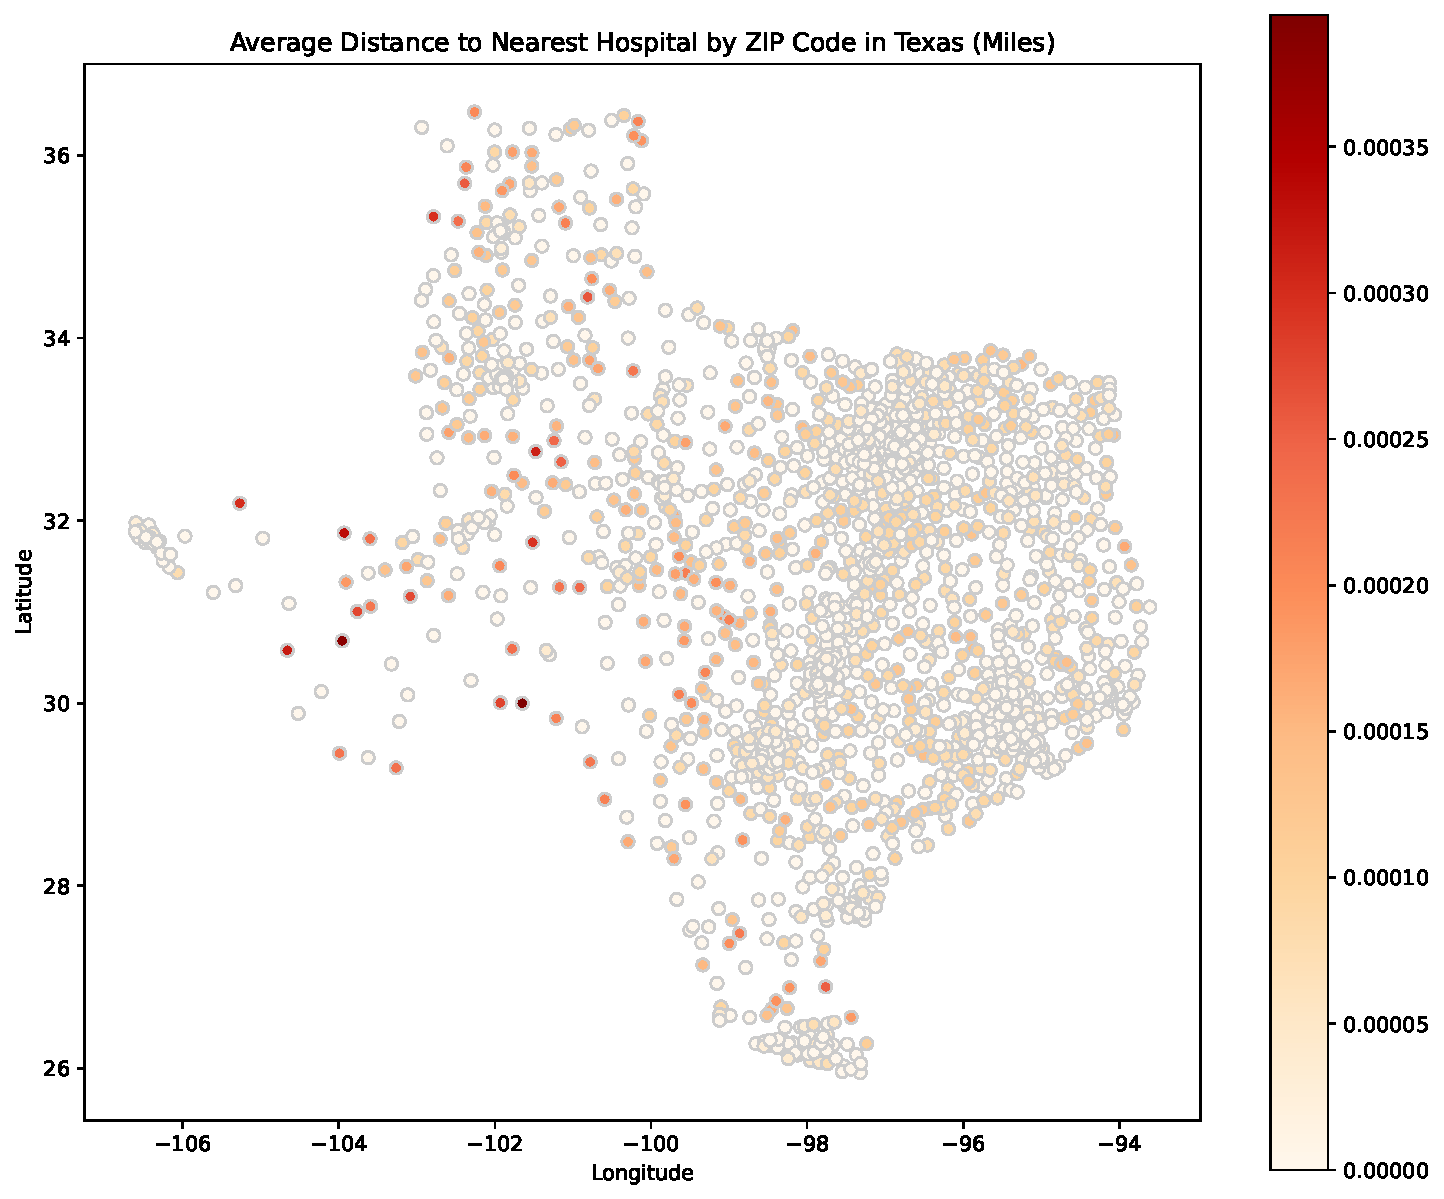
\includegraphics{pset4_template_files/figure-pdf/cell-21-output-2.pdf}

\subsection{Effects of closures on access in Texas (15
pts)}\label{effects-of-closures-on-access-in-texas-15-pts}

\begin{enumerate}
\def\labelenumi{\arabic{enumi}.}
\tightlist
\item
\end{enumerate}

\begin{Shaded}
\begin{Highlighting}[]
\NormalTok{texas\_closures }\OperatorTok{=}\NormalTok{ confirmed\_closures[confirmed\_closures[}\StringTok{\textquotesingle{}ZIP\_CD\textquotesingle{}}\NormalTok{].astype(}
    \BuiltInTok{str}\NormalTok{).}\BuiltInTok{str}\NormalTok{.startswith((}\StringTok{\textquotesingle{}75\textquotesingle{}}\NormalTok{, }\StringTok{\textquotesingle{}76\textquotesingle{}}\NormalTok{, }\StringTok{\textquotesingle{}77\textquotesingle{}}\NormalTok{, }\StringTok{\textquotesingle{}78\textquotesingle{}}\NormalTok{, }\StringTok{\textquotesingle{}79\textquotesingle{}}\NormalTok{))]}
\NormalTok{closures\_by\_zipcode }\OperatorTok{=}\NormalTok{ texas\_closures[}\StringTok{\textquotesingle{}ZIP\_CD\textquotesingle{}}\NormalTok{].value\_counts().reset\_index()}
\NormalTok{closures\_by\_zipcode.columns }\OperatorTok{=}\NormalTok{ [}\StringTok{\textquotesingle{}ZIP Code\textquotesingle{}}\NormalTok{, }\StringTok{\textquotesingle{}Number of Closures\textquotesingle{}}\NormalTok{]}

\NormalTok{closures\_by\_zipcode}
\end{Highlighting}
\end{Shaded}

\begin{longtable}[]{@{}lll@{}}
\toprule\noalign{}
& ZIP Code & Number of Closures \\
\midrule\noalign{}
\endhead
\bottomrule\noalign{}
\endlastfoot
0 & 77380.0 & 2 \\
1 & 78205.0 & 1 \\
\end{longtable}

\begin{enumerate}
\def\labelenumi{\arabic{enumi}.}
\setcounter{enumi}{1}
\tightlist
\item
\end{enumerate}

\begin{Shaded}
\begin{Highlighting}[]
\NormalTok{affected\_zip\_codes }\OperatorTok{=}\NormalTok{ confirmed\_closures[confirmed\_closures[}\StringTok{\textquotesingle{}ZIP\_CD\textquotesingle{}}\NormalTok{].astype(}
    \BuiltInTok{str}\NormalTok{).}\BuiltInTok{str}\NormalTok{.startswith(}\StringTok{\textquotesingle{}7\textquotesingle{}}\NormalTok{)][}\StringTok{\textquotesingle{}ZIP\_CD\textquotesingle{}}\NormalTok{].unique()}
\NormalTok{affected\_zip\_df }\OperatorTok{=}\NormalTok{ pd.DataFrame(affected\_zip\_codes, columns}\OperatorTok{=}\NormalTok{[}\StringTok{\textquotesingle{}ZCTA5\textquotesingle{}}\NormalTok{])}
\NormalTok{affected\_zip\_df[}\StringTok{\textquotesingle{}affected\textquotesingle{}}\NormalTok{] }\OperatorTok{=} \DecValTok{1}

\NormalTok{zips\_texas\_centroids[}\StringTok{\textquotesingle{}ZCTA5\textquotesingle{}}\NormalTok{] }\OperatorTok{=}\NormalTok{ zips\_texas\_centroids[}\StringTok{\textquotesingle{}ZCTA5\textquotesingle{}}\NormalTok{].astype(}
    \BuiltInTok{str}\NormalTok{).fillna(}\StringTok{\textquotesingle{}\textquotesingle{}}\NormalTok{)}
\NormalTok{affected\_zip\_df[}\StringTok{\textquotesingle{}ZCTA5\textquotesingle{}}\NormalTok{] }\OperatorTok{=}\NormalTok{ affected\_zip\_df[}\StringTok{\textquotesingle{}ZCTA5\textquotesingle{}}\NormalTok{].astype(}\BuiltInTok{str}\NormalTok{).fillna(}\StringTok{\textquotesingle{}\textquotesingle{}}\NormalTok{)}
\NormalTok{zips\_texas\_affected }\OperatorTok{=}\NormalTok{ zips\_texas\_centroids.merge(}
\NormalTok{    affected\_zip\_df, on}\OperatorTok{=}\StringTok{\textquotesingle{}ZCTA5\textquotesingle{}}\NormalTok{, how}\OperatorTok{=}\StringTok{\textquotesingle{}left\textquotesingle{}}\NormalTok{)}
\NormalTok{zips\_texas\_affected[}\StringTok{\textquotesingle{}affected\textquotesingle{}}\NormalTok{] }\OperatorTok{=}\NormalTok{ zips\_texas\_affected[}\StringTok{\textquotesingle{}affected\textquotesingle{}}\NormalTok{].fillna(}
    \DecValTok{0}\NormalTok{)  }\CommentTok{\# Fill NaN values with 0 (unaffected)}

\NormalTok{num\_directly\_affected\_zips }\OperatorTok{=} \BuiltInTok{len}\NormalTok{(affected\_zip\_codes)}
\BuiltInTok{print}\NormalTok{(}
    \SpecialStringTok{f"Number of directly affected ZIP codes in Texas: }\SpecialCharTok{\{}\NormalTok{num\_directly\_affected\_zips}\SpecialCharTok{\}}\SpecialStringTok{"}\NormalTok{)}
\end{Highlighting}
\end{Shaded}

\begin{verbatim}
Number of directly affected ZIP codes in Texas: 3
\end{verbatim}

\begin{verbatim}
/opt/anaconda3/lib/python3.11/site-packages/geopandas/geodataframe.py:1819: SettingWithCopyWarning:


A value is trying to be set on a copy of a slice from a DataFrame.
Try using .loc[row_indexer,col_indexer] = value instead

See the caveats in the documentation: https://pandas.pydata.org/pandas-docs/stable/user_guide/indexing.html#returning-a-view-versus-a-copy
\end{verbatim}

\begin{enumerate}
\def\labelenumi{\arabic{enumi}.}
\setcounter{enumi}{2}
\tightlist
\item
\end{enumerate}

\begin{Shaded}
\begin{Highlighting}[]
\NormalTok{buffer\_distance }\OperatorTok{=} \DecValTok{10} \OperatorTok{*} \FloatTok{1609.34}
\NormalTok{zips\_texas\_centroids }\OperatorTok{=}\NormalTok{ zips\_texas\_centroids.to\_crs(epsg}\OperatorTok{=}\DecValTok{3857}\NormalTok{)}

\NormalTok{affected\_zip\_codes }\OperatorTok{=}\NormalTok{ confirmed\_closures[confirmed\_closures[}\StringTok{\textquotesingle{}ZIP\_CD\textquotesingle{}}\NormalTok{].astype(}
    \BuiltInTok{str}\NormalTok{).}\BuiltInTok{str}\NormalTok{.startswith(}\StringTok{\textquotesingle{}7\textquotesingle{}}\NormalTok{)][}\StringTok{\textquotesingle{}ZIP\_CD\textquotesingle{}}\NormalTok{].unique()}
\NormalTok{directly\_affected\_gdf }\OperatorTok{=}\NormalTok{ zips\_texas\_centroids[zips\_texas\_centroids[}\StringTok{\textquotesingle{}ZCTA5\textquotesingle{}}\NormalTok{].isin(}
\NormalTok{    affected\_zip\_codes)]}

\NormalTok{directly\_affected\_buffer }\OperatorTok{=}\NormalTok{ directly\_affected\_gdf.copy()}
\NormalTok{directly\_affected\_buffer[}\StringTok{\textquotesingle{}geometry\textquotesingle{}}\NormalTok{] }\OperatorTok{=}\NormalTok{ directly\_affected\_buffer.geometry.}\BuiltInTok{buffer}\NormalTok{(}
\NormalTok{    buffer\_distance)}

\NormalTok{zips\_texas\_centroids }\OperatorTok{=}\NormalTok{ zips\_texas\_centroids.to\_crs(}
\NormalTok{    directly\_affected\_buffer.crs)}
\NormalTok{indirectly\_affected\_gdf }\OperatorTok{=}\NormalTok{ gpd.sjoin(}
\NormalTok{    zips\_texas\_centroids, directly\_affected\_buffer, how}\OperatorTok{=}\StringTok{\textquotesingle{}inner\textquotesingle{}}\NormalTok{, predicate}\OperatorTok{=}\StringTok{\textquotesingle{}intersects\textquotesingle{}}\NormalTok{)}

\NormalTok{indirectly\_affected\_gdf }\OperatorTok{=}\NormalTok{ indirectly\_affected\_gdf[}\OperatorTok{\textasciitilde{}}\NormalTok{indirectly\_affected\_gdf[}\StringTok{\textquotesingle{}ZCTA5\_left\textquotesingle{}}\NormalTok{].isin(}
\NormalTok{    affected\_zip\_codes)]}
\NormalTok{num\_indirectly\_affected\_zips }\OperatorTok{=}\NormalTok{ indirectly\_affected\_gdf[}\StringTok{\textquotesingle{}ZCTA5\_left\textquotesingle{}}\NormalTok{].nunique()}

\BuiltInTok{print}\NormalTok{(}
    \SpecialStringTok{f"Number of indirectly affected ZIP codes in Texas: }\SpecialCharTok{\{}\NormalTok{num\_indirectly\_affected\_zips}\SpecialCharTok{\}}\SpecialStringTok{"}\NormalTok{)}
\end{Highlighting}
\end{Shaded}

\begin{verbatim}
Number of indirectly affected ZIP codes in Texas: 0
\end{verbatim}

\begin{enumerate}
\def\labelenumi{\arabic{enumi}.}
\setcounter{enumi}{3}
\tightlist
\item
\end{enumerate}

\begin{Shaded}
\begin{Highlighting}[]
\NormalTok{zips\_texas\_centroids[}\StringTok{\textquotesingle{}Category\textquotesingle{}}\NormalTok{] }\OperatorTok{=} \StringTok{\textquotesingle{}Not Affected\textquotesingle{}}
\NormalTok{zips\_texas\_centroids.loc[zips\_texas\_centroids[}\StringTok{\textquotesingle{}ZCTA5\textquotesingle{}}\NormalTok{].isin(}
\NormalTok{    affected\_zip\_codes), }\StringTok{\textquotesingle{}Category\textquotesingle{}}\NormalTok{] }\OperatorTok{=} \StringTok{\textquotesingle{}Directly Affected\textquotesingle{}}
\NormalTok{indirectly\_affected\_zip\_codes }\OperatorTok{=}\NormalTok{ indirectly\_affected\_gdf[}\StringTok{\textquotesingle{}ZCTA5\_left\textquotesingle{}}\NormalTok{].unique()}
\NormalTok{zips\_texas\_centroids.loc[zips\_texas\_centroids[}\StringTok{\textquotesingle{}ZCTA5\textquotesingle{}}\NormalTok{].isin(}
\NormalTok{    indirectly\_affected\_zip\_codes), }\StringTok{\textquotesingle{}Category\textquotesingle{}}\NormalTok{] }\OperatorTok{=} \StringTok{\textquotesingle{}Indirectly Affected\textquotesingle{}}

\NormalTok{fig, ax }\OperatorTok{=}\NormalTok{ plt.subplots(}\DecValTok{1}\NormalTok{, }\DecValTok{1}\NormalTok{, figsize}\OperatorTok{=}\NormalTok{(}\DecValTok{12}\NormalTok{, }\DecValTok{10}\NormalTok{))}
\NormalTok{zips\_texas\_centroids.plot(}
\NormalTok{    column}\OperatorTok{=}\StringTok{\textquotesingle{}Category\textquotesingle{}}\NormalTok{,}
\NormalTok{    cmap}\OperatorTok{=}\StringTok{\textquotesingle{}Set1\textquotesingle{}}\NormalTok{,}
\NormalTok{    ax}\OperatorTok{=}\NormalTok{ax,}
\NormalTok{    legend}\OperatorTok{=}\VariableTok{True}\NormalTok{,}
\NormalTok{    legend\_kwds}\OperatorTok{=}\NormalTok{\{}\StringTok{\textquotesingle{}title\textquotesingle{}}\NormalTok{: }\StringTok{"ZIP Code Categories"}\NormalTok{\}}
\NormalTok{)}
\NormalTok{plt.title(}\StringTok{\textquotesingle{}Texas ZIP Codes by Impact from Hospital Closures (2016{-}2019)\textquotesingle{}}\NormalTok{)}
\NormalTok{plt.xlabel(}\StringTok{\textquotesingle{}Longitude\textquotesingle{}}\NormalTok{)}
\NormalTok{plt.ylabel(}\StringTok{\textquotesingle{}Latitude\textquotesingle{}}\NormalTok{)}
\NormalTok{plt.show()}
\end{Highlighting}
\end{Shaded}

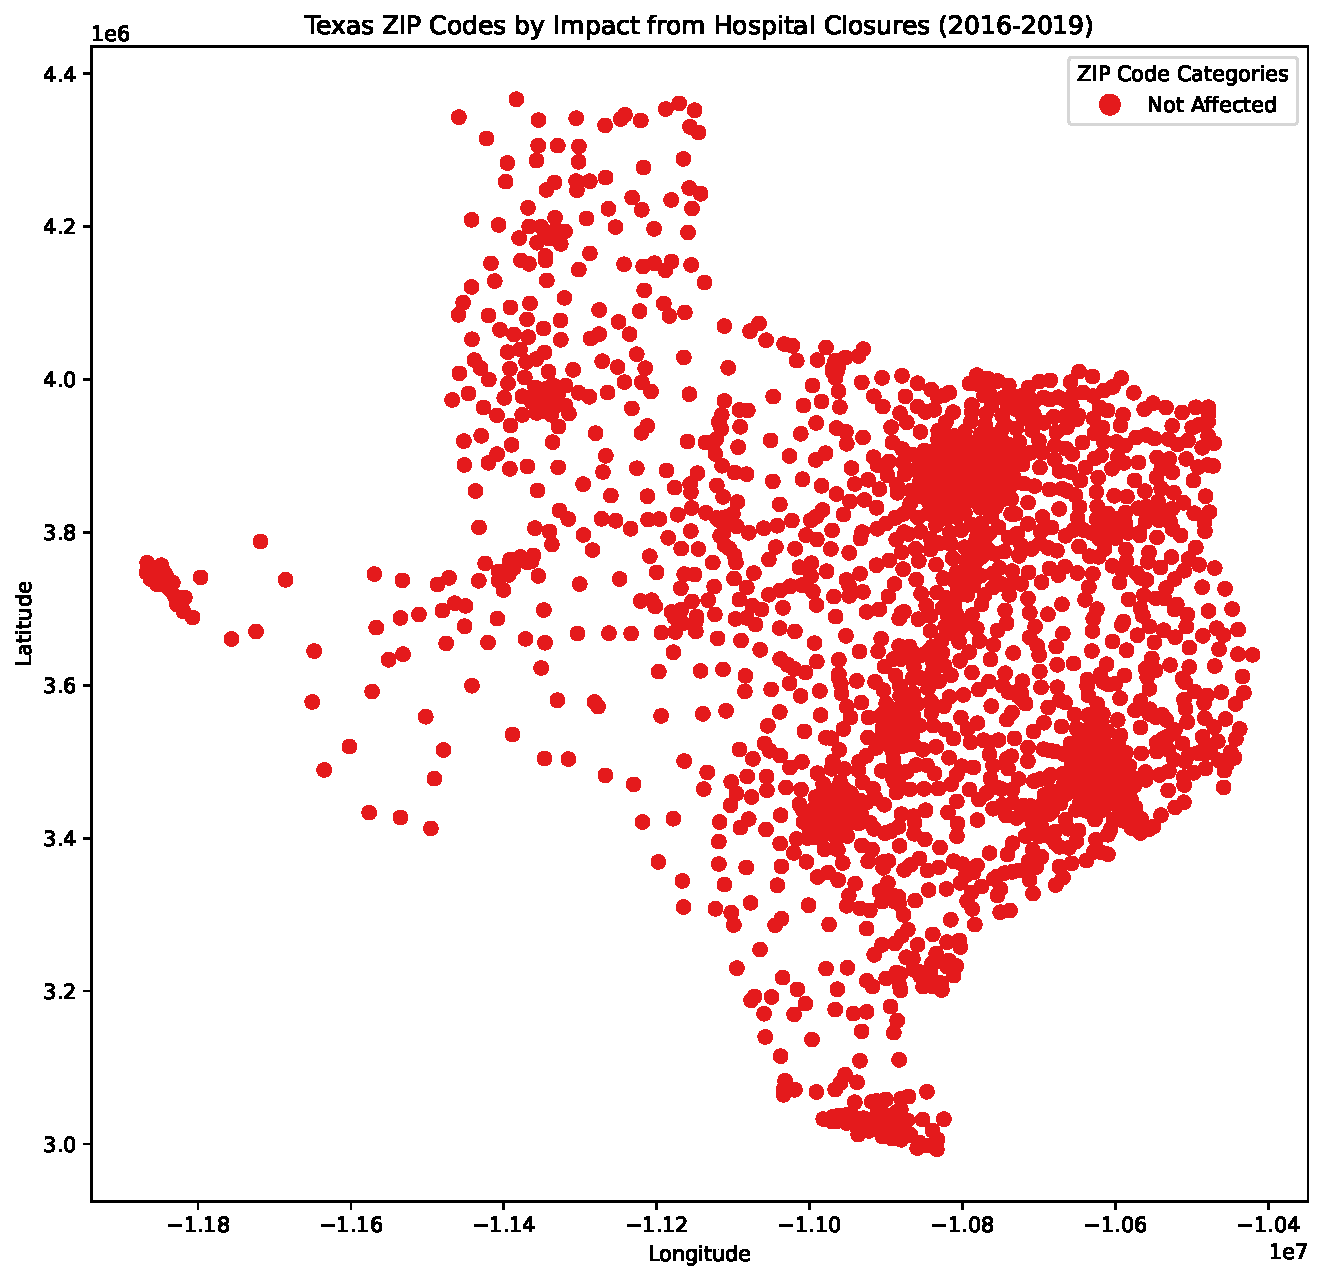
\includegraphics{pset4_template_files/figure-pdf/cell-25-output-1.pdf}

\subsection{Reflecting on the exercise (10
pts)}\label{reflecting-on-the-exercise-10-pts}

\begin{enumerate}
\def\labelenumi{\arabic{enumi}.}
\tightlist
\item
  A significant drawback of the ``first-pass'' approach to identifying
  hospital closures is the risk of misclassifying institutions that
  experience temporary closures or suspensions as permanently closed.
  These facilities may temporarily close for repairs or financial
  reasons, thereafter reopening; however, this process could mistakenly
  classify them as permanently closed. Another concern is the potential
  for mistaken classification resulting from mergers or acquisitions,
  wherein a hospital may operate under a new name or certification
  number while appearing ``closed'' in the data. To mitigate these
  limitations, a more precise strategy would involve integrating
  supplementary data sources, such as state health department records or
  local news, to cross-verify and validate closures. Furthermore, the
  implementation of geographic proximity tracking would assist in
  determining whether hospitals that appear ``closed'' have just
  relocated or amalgamated with adjacent facilities, hence minimizing
  misclassification.
\item
  One limitation of this approach is that it only looks at hospital
  closures within each specific ZIP code, without considering hospitals
  in nearby ZIP codes. This means that if a hospital closes in a ZIP
  code, but there is still another hospital close by in a neighboring
  ZIP code, people might still have access to hospital services, so the
  closure might not have a big impact on them. On the other hand, if a
  hospital closes in a ZIP code and there are no other hospitals nearby,
  people in that area could lose easy access to healthcare, and the
  impact of the closure would be much greater. In addition, not all ZIP
  codes have the same number of people living in them, and not every
  area needs the same amount of healthcare. If a hospital closes in a
  ZIP code where a lot of people live, it could have a bigger effect
  because more people depend on that hospital for healthcare. But if a
  hospital closes in a ZIP code with fewer people, the impact might be
  smaller since not as many people rely on that hospital for their
  healthcare needs. Some suggests to improve this measure: rather than
  simply counting how many hospitals closed in each ZIP code, we could
  measure the distance from each ZIP code to the nearest hospital both
  before and after the closures took place (from 2016 to 2019). This
  would help us see if people in each ZIP code now have to travel
  farther to reach a hospital after the closures. We should also
  consider population-weighted calculations to quantify how population
  plays a role in the impact of hospital closures.
\end{enumerate}




\end{document}
